\chapter{Coordinates}
\label{s:coords}
\index{coordinates|hyperbf}

\vspace*{-0.3in}
\bmad uses three coordinate systems as illustrated in \fig{f:coords}. First, the \vn{global} (also
called ``\vn{floor}'') coordinates are independent of the placement accelerator. Things such as the
building the accelerator is in may be described using \vn{global} coordinates.

\begin{figure}[!b]
  \centering
  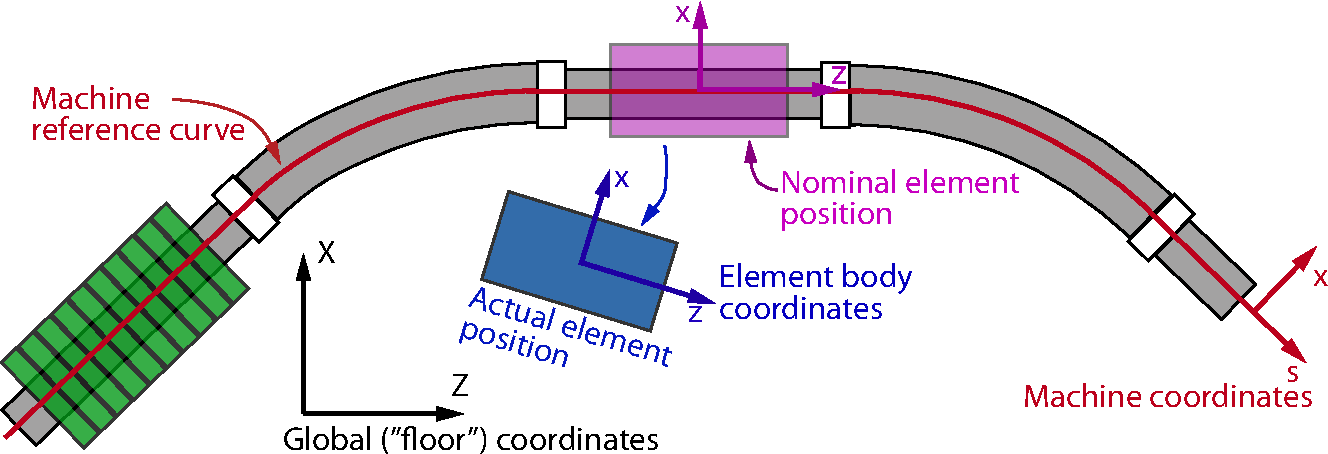
\includegraphics[width=5.0in]{coordinates.pdf}
  \caption[The three coordinate system used by \bmad.]
{The \vn{global} (or ``\vn{floor}'') coordinate system
is independent of the accelerator.  The \vn{machine} curvilinear coordinate system follows the bends
of the accelerator.  Each lattice element has \vn{element body} coordinates which, if the element is
not ``misaligned'' is the same as the \vn{machine} coordinates. 
The $x=y=0$ curved line of the
machine coordinate system is known as the ``reference orbit''.}
  \label{f:coords}
\end{figure}

It is inconvenient to describe the position of a particle beam using the 
\vn{global} coordinate system so
a ``\vn{machine}'' coordinate system is used (\sref{s:machine.coords}).  This curvilinear coordinate
system defines the nominal position of the lattice elements.  The relationship between the
\vn{machine} and \vn{global} coordinate systems is described in \sref{s:global}.

The ``nominal'' position of a lattice element is the position of the element without any
position and orientation shifts (\sref{s:align.g}) 
which are sometimes referred to as ``misalignments''. 
Each lattice element has ``\vn{element body}'' (or just ``\vn{body}'') 
coordinates which are attached to the physical element and the electric and magnetic
fields of an element are described with respect to \vn{body} coordinates.  If there are no
misalignments, the \vn{body} coordinates are aligned with the 
\vn{machine} coordinates.
The transformation between \vn{machine} and \vn{body} coordinates is given in
\sref{s:lab.body.transform}.
The $x=y=0$ curved line of the
machine coordinate system is known as the ``\vn{reference orbit}''.

%-----------------------------------------------------------------------------
\section{Machine Coordinates and Reference Orbit}
\label{s:machine.coords}

%-----------------------------------------------------------------------------
\subsection{The Reference Orbit}
\label{s:ref}
\index{reference orbit|hyperbf}
\index{machine coordinates|hyperbf}

\begin{figure}[tb]
  \centering
  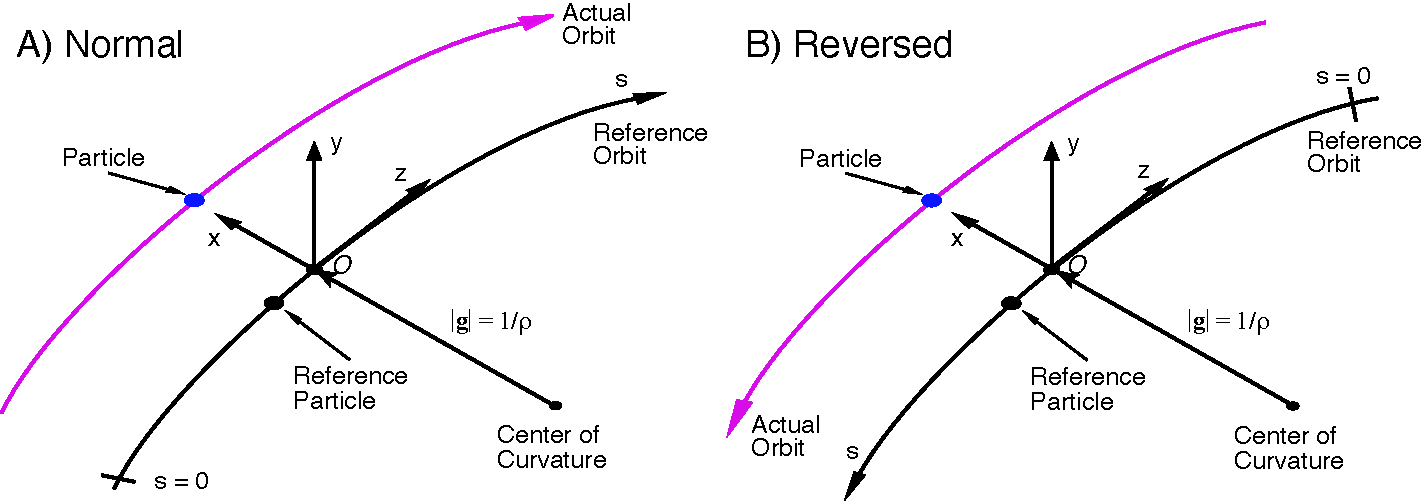
\includegraphics[width=6in]{machine-coords.pdf}
  \caption[Reference coordinate system.]
{The reference coordinate system. By construction, a particle's $z$ coordinate is zero.  This
is not to be confused with the phase space $z$ coordinate (\sref{s:phase.space}). The curvature
vector $\bfg$ lies in the $x$-$y$ plane and has a magnitude of $1/\rho$ where $\rho$ is the bending
radius. A) The $z$-axis will normally be parallel to the $s$-axis. B) For \vn{reversed} elements it
will be antiparallel. In both cases, the particle and reference particle are traveling in the
direction of greater $s$.}
  \label{f:machine.coords}
\end{figure}

The \vn{machine reference orbit} is the curved path used to define a coordinate system for describing
a particle's position as shown in \fig{f:machine.coords}. The reference orbit is also used for
orientating lattice elements in space. At a given time $t$, a particle's position can be described
by a point $\calO$ on the reference orbit a distance $s$ relative to the reference orbit's zero
position plus a transverse $(x,y)$ offset. The point $\calO$ on the reference orbit is used as the
origin of the machine $(x, y, z)$ coordinate system with the $z$--axis tangent to the reference
orbit. The $z$--axis will generally be pointing in the direction of increasing $s$
(\fig{f:machine.coords}A) but, as discussed below, will point counter to $s$ for elements that are
longitudinally \vn{reversed} in orientation (\fig{f:machine.coords}B). 
The $x$ and $y$--axes are perpendicular to the reference
orbit and, by construction, the particle is always at $z = 0$. The coordinate system so constructed
is called the \vn{``machine coordinate system''} when there is need to distinguish it from the 
\vn{``element body coordinate system''}
(\sref{s:coords}) which is attached to the physical element. There is a separate reference orbit
for each branch (\sref{s:branch.def}) of a lattice.

\index{x_offset}\index{y_offset}
\index{x_rot}\index{y_rot}\index{wiggler}
The reference orbit may not correspond to the orbit that any actual particle could travel.
A common example is the \vn{wiggler} element where particles always oscillate about the reference
orbit which is a straight line.

Do not confuse this reference orbit (which defines the machine coordinate system) with the reference
orbit about which the transfer maps are calculated (\sref{s:twiss}). The former is fixed by the
lattice while the latter can be any arbitrary orbit.

%-----------------------------------------------------------------------------
\subsection{Element Entrance and Exit Coordinates}
\label{s:ent.exi}
\index{element body coordinates}

%--------------------------------------

  \begin{figure}[tb]
  \centering
  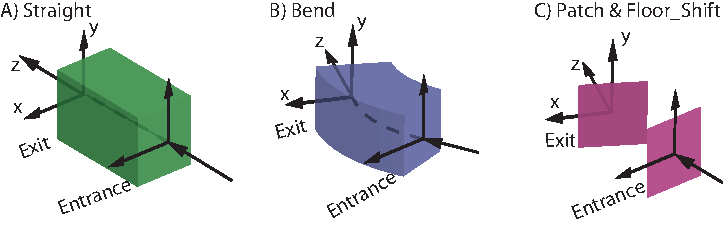
\includegraphics[width=5in]{ele-coord-frame.pdf}
\caption[Lattice elements as LEGO blocks.]{Lattice elements can be imagined as ``LEGO blocks'' which
fit together to form the reference orbit along with the machine coordinate system. How elements
join together is determined in part by their entrance and exit coordinate frames. A) For
straight line elements the entrance and exit frames are colinear. B) For bends elements, the two
frames are rotated with respect to each other. C) For \vn{patch} and \vn{floor_shift} elements the
exit frame may be arbitrarily positioned with respect to the entrance frame.}
  \label{f:ele.coord.frame}
  \end{figure}

%--------------------------------------

\index{sbend}\index{rbend}
\index{crystal}\index{mirror}\index{entrance_end}
\index{exit_end}\index{patch}\index{floor_shift}
One way of thinking about the reference orbit and the machine coordinates is to imagine that each
element is like a LEGO block with an ``\vn{entrance}'' and an ``\vn{exit}'' coordinate frame as
illustrated in \fig{f:ele.coord.frame}\footnote
  {
Thanks to Dan Abell for this analogy.
  }. 
These coordinate frames are attached to the element. that is, things like electric and magnetic
fields, apertures, etc., are described with respect to the entrance and exit coordinates.  Thus, for
example, the \vn{e1} edge of a bend (\sref{s:bend}) is always at the \vn{entrance} face and the
\vn{e2} is always at the \vn{exit} face. Most elements have a ``straight'' geometry as shown in
\fig{f:ele.coord.frame}A. That is, the reference orbit through the element is a straight line
segment with the $x$ and $y$ axes always pointing in the same direction.  For a \vn{bend} element
(\sref{s:bend}), the reference orbit is a segment of a circular arc as shown in
\fig{f:ele.coord.frame}B. With the \vn{ref_tilt} parameter of a bend set to zero, the rotation axis
between the entrance and exit frames is parallel to the $y$-axis (\sref{s:global}). For \vn{patch}
(\sref{s:patch}), and \vn{floor_shift} (\sref{s:floor.ele}) elements, the exit face can can
arbitrarily oriented with respect to the entrance end. In this case, the reference orbit between the
entrance and exit faces is not defined.

%-----------------------------------------------------------------------------
\subsection{Reference Orbit and Machine Coordinates Construction}
\label{s:ref.construct}
\index{reference orbit!construction}
\index{upstream element end}\index{downstream element end}
\index{entrance element end}\index{exit element end}

%-----------------------------------------------------------------------------
\begin{figure}[tb]
  \centering
  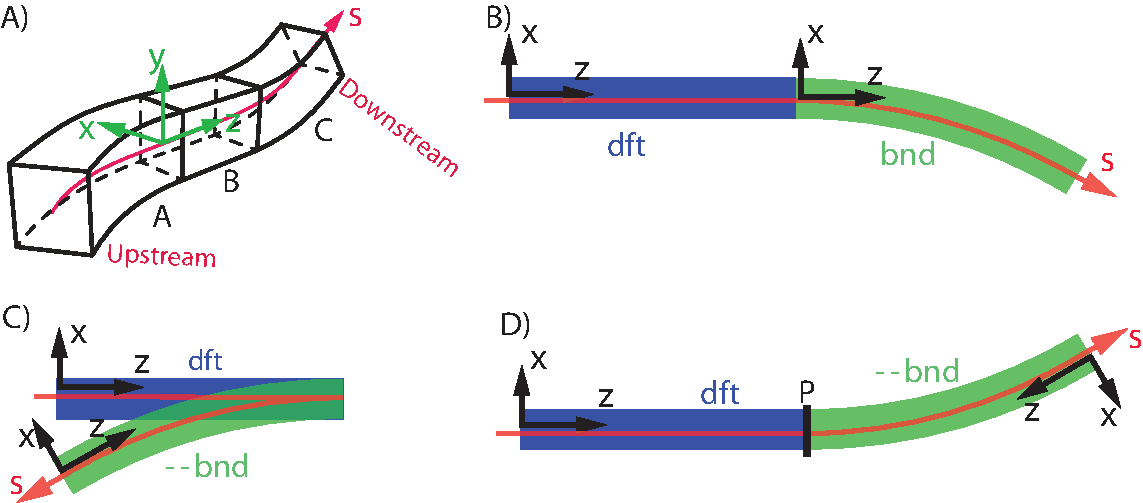
\includegraphics[width=5in]{patch-between.pdf}
  \caption[Machine coordinates construction.]{A) The machine coordinates are constructed by
connecting the \vn{downstream} reference frame of one element with the \vn{upstream} reference frame
of the next element in the branch. Coordinates shown is for the mating of element \vn{A} to element
{B}.  B) Example with drift element \vn{dft} followed by a bend \vn{bnd}. Both elements are
unreversed. C) Similar to (B) but in this case element \vn{bnd} is reversed.  D) Similar to (C) but
in this case a reflection patch has been added in between \vn{dft} and \vn{bnd}.  In (B), (C), and
(D) the $(x,z)$ coordinates are drawn at the \vn{entrance} end of the elements. The $y$ coordinate
is always out of the page.}
  \label{f:patch.between}
\end{figure}
%-----------------------------------------------------------------------------

\index{root branch}
Assuming for the moment that there are no \vn{fiducial} elements present, the construction of the
reference orbit starts at the \vn{beginning_ele} element (\sref{s:begin.ele}) at the start of a
branch. If the branch is a \vn{root} branch (\sref{s:lattice.def}), The orientation of the beginning
element within the global coordinate system (\sref{s:coords}) can be set via the appropriate
positioning statements (\sref{s:beginning}). If the branch is not a \vn{root} branch, the position
of the beginning element is determined by the position of the \vn{fork} or \vn{photon_fork} element
from which the branch forks from. Unless set otherwise in the lattice file, $s = 0$ at the
\vn{beginning_ele} element.

If there are \vn{fiducial} elements, the machine coordinates are constructed beginning at these
elements.

Once the beginning element in a branch is positioned, succeeding elements are concatenated together
to form the machine coordinates. All elements have an ``\vn{upstream}'' and a ``\vn{downstream}''
end as shown in \fig{f:patch.between}A. The \vn{downstream} end of an element is always farther (at
greater $s$) from the beginning element than the \vn{upstream} end of the element.  Particles travel
in the $+s$ direction, so particles will enter an element at the upstream end and exit at the
downstream end.

Normally, the \vn{upstream} end is the same as the element's \vn{entrance} end 
(\fig{f:ele.coord.frame}) and the
\vn{downstream} end is the same as the element's \vn{exit} end. However, if an element is reversed
(\sref{s:ele.reverse}), the element's \vn{exit} end will be \vn{upstream} end and the element's
\vn{entrance} end will be the \vn{downstream} end. That is, for a reversed element, particles 
traveling downstream will
enter at the element's \vn{exit} end and will exit at the \vn{entrance} end.

The procedure to connect elements together to form the machine coordinates is to mate the
downstream reference frame of the element with the upstream reference frame of the next element in
the branch so that, without misalignments, the $(x,y,z)$ axes coincide\footnote
  {
If there are misalignments, the \vn{entrance} and \vn{exit} frames will move with the element. However,
the \vn{upstream} and \vn{downstream} frames, along with the reference orbit and machine
coordinates, will not move.
  }. 
This is illustrated in \fig{f:patch.between}. \fig{f:patch.between}A shows the general situation
with the downstream frame of element \vn{A} mated to the upstream frame of element \vn{B}.
Figures~\ref{f:patch.between}B-C show branches constructed from the following lattice file:
\begin{example}
  @ele dft = drift(L = 2)
  @ele bnd = bend(l = 2, g = pi/12)
  @ele p = patch(x_rot = pi)                   ! Reflection patch.
  BL = beamline("BL", [dft, bnd])              ! No reversal.
  CL = beamline("CL", [dft, reverse(bnd)])     ! Illegal. Do not use!
  DL = beamline("DL", [dft, p, reverse(bnd)])  ! Valid.
\end{example}
The $(x,z)$ coordinates are drawn at the entrance end of the elements and $z$ will always point
towards the element's exit end.  \fig{f:patch.between}B shows the branch constructed from
\vn{BL} containing an unreversed drift named \vn{dft} connected to an unreversed bend named
\vn{bnd}. \fig{f:patch.between}C shows the branch constructed from \vn{CL}. This is like
\vn{BL} except here element \vn{bnd} is reversed. This gives an unphysical situation since a
particle traveling through \vn{dft} will ``fall off'' when it gets to the end.
\fig{f:patch.between}D shows the branch constructed from \vn{DL}. Here a ``\vn{reflection}''
patch \vn{P} (\sref{s:reflect.patch}) has been added to get a plausible geometry. The patch rotates the
coordinate system around the $y$-axis by 180\Deg (leaving the $y$-axis invariant). It is always the
case that a reflection patch is needed between reversed and unreversed elements

Notes:
\begin{itemize}
\item
If the first element after the \vn{beginning_ele} element at the start of a branch is reversed, the
\vn{beginning_ele} element will be marked as reversed so that a reflection patch is not needed in
this circumstance.
\item
Irrespective of whether elements are reversed or not, the machine $(x,y,z)$ coordinate system
at all $s$-positions will always be a right-handed coordinate system.
\item
Care must be take when using reversed elements. For example, if the field of the \vn{bnd} element in
\vn{B_line} is appropriate for, say, electrons, that is, electrons will be bent in a clockwise
fashion going through \vn{bnd}, then an electron going through \vn{D_line} will be lost in the bend
(the $y$-axis and hence the field is in the same direction for both cases so electrons will still be
bent in a clockwise fashion but with \vn{D_line} a particle needs to be bent counterclockwise to get
through the bend). To get a particle through the bend, positrons must be used.
\item
A reflection patch that rotated the coordinates, for example, around the $x$-axis by 180\Deg (by
setting \vn{x_rot} to \vn{pi}) would also produce a plausible geometry.
\end{itemize}

%-----------------------------------------------------------------------------

\begin{figure}[bt]
  \centering
  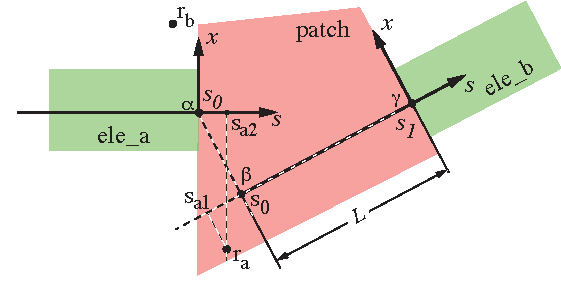
\includegraphics[width=5in]{patch-problem.pdf}
  \caption[The machine reference coordinates in a \vn{patch} element.]
{The machine reference coordinates in a \vn{Patch} element. The \vn{patch} element, shown
schematically as an irregular quadrilateral, is sandwiched between elements \vn{ele_a} and
\vn{ele_b}. \vn{L} is the length of the \vn{patch}. In this example, the \vn{patch} has a finite
\vn{y_rot}.}
  \label{f:patch.prob}
\end{figure}

%-----------------------------------------------------------------------------
%-----------------------------------------------------------------------------
\subsection{Patch Element Coordinates}
\label{s:patch.prob}
\index{patch}

Generally, if a particle is reasonably near the reference orbit, there is a one-to-one mapping
between the particle's position and $(x, y, s)$ coordinates. A \vn{patch} (\sref{s:patch}) elements
with a non-zero \vn{x_rot} or non-zero \vn{y_rot} breaks the one-to-one mapping. This is
illustrated in \fig{f:patch.prob}.  The \vn{patch} element, shown schematically as an, irregular
quadrilateral, is sandwiched between elements \vn{ele_a} and \vn{ele_b}. The machine coordinate system
with origin at $\alpha$ are the coordinates at the end of \vn{ele_a}. The coordinates at the end of
the \vn{patch} has its origin labeled $\gamma$. By convention, the length of the patch \vn{L} is
taken to be the longitudinal distance from $\alpha$ to $\gamma$ with the \vn{patch}'s exit
coordinates defining the longitudinal direction. The ``beginning'' point of the \vn{patch} on the
reference orbit a distance \vn{L} from point $\gamma$ is labeled $\beta$ in the figure.

In the machine $(x, y, s)$ coordinate system a particle at $\alpha$ will have some value $s = s_0$. A
particle at point $\beta$ will have the same value $s = s_0$ and a particle at $\gamma$ will have $s
= s_1 = s_0 + L$. A particle at point $r_a$ in \fig{f:patch.prob} illustrates the problem of
assigning $(x, y, s)$ coordinates to a given position. If the particle is considered to be within
the region of \vn{ele_a}, the particle's $s$ position will be $s_{a2}$ which is greater than the
value $s_0$ at the exit end of the element. This contradicts the expectation that particles within
\vn{ele_a} will have $s \le s_0$.  If, on the other hand, the particle is considered to be within
the \vn{patch} region, the particle's $s$ position will be $s_{a1}$ which is less than the value
$s_0$ at the entrance to the patch. This contradicts the expectation that a particles within the
\vn{patch} will have $s \ge s_0$.

To resolve this problem, \bmad considers a particle at position $r_a$ to be within the \vn{patch}
region. This means that there is, in theory, no lower limit to the $s$-position that a particle in
the \vn{patch} region can have. This also implies that there is a discontinuity in the $s$-position
of a particle crossing the exit face of \vn{ele1}. Typically, when particles are translated from the
exit face of one element to the exit face of the next, this \vn{patch} problem does not appear. It
only appears when the track between faces is considered.

Notice that a particle at position $r_b$ in \fig{f:patch.prob} can simultaneously be considered to
be in either \vn{ele_a} or the \vn{patch}. While this creates an ambiguity it does not complicate
tracking.

%-----------------------------------------------------------------------------
\section{Global Coordinates}
\label{s:global}
\index{global coordinates|hyperbf}

\begin{figure}[tb]
  \centering
  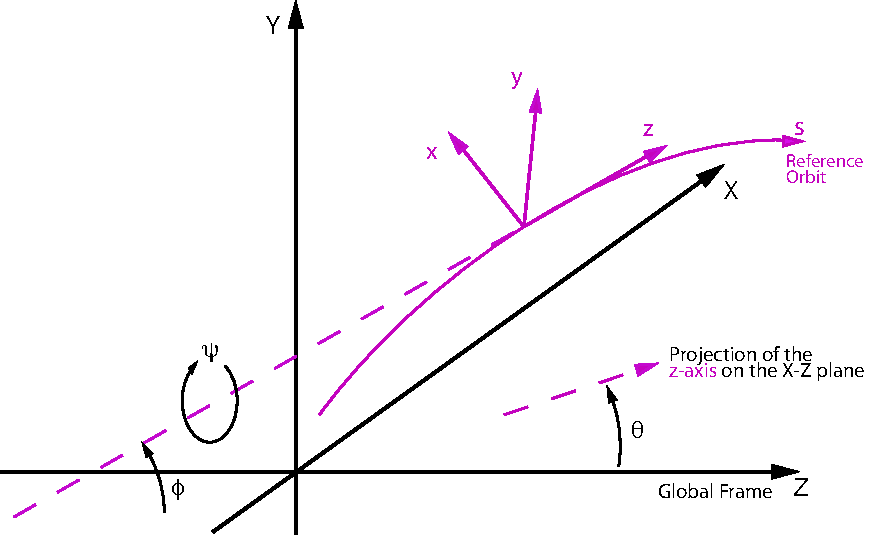
\includegraphics{global-coords.pdf}
  \caption[The Global Coordinate System]{
The machine (reference) coordinate system (purple), which is a function of $s$ along the reference
orbit, is described in the global coordinate system (black) by a position $(X(s), Y(s), Z(s))$ and
and by angles $\theta(s)$, $\phi(s)$, and $\psi(s)$.
  }
  \label{f:global.coords}
\end{figure}

The Cartesian \vn{global} coordinate system, also called the `floor'' coordinate system, is the
coordinate system ``attached to the earth'' that is used to describe the machine coordinate
system. Following the \mad\ convention, the \vn{global} coordinate axis are labeled $(X, Y,
Z)$. Conventionally, $Y$ is the ``vertical'' coordinate and $(X, Z)$ are the ``horizontal''
coordinates. To describe how the machine coordinate system is oriented within the global coordinate
system, each point on the $s$-axis of the machine coordinate system is characterized by its $(X, Y,
Z)$ position and by three angles $\theta(s)$, $\phi(s)$, and $\psi(s)$ that describe the orientation
of the machine coordinate axes as shown in \fig{f:global.coords}. These three angles are defined as
follows:
\begin{description}
%
\item[$\theta(s)$ Azimuth (yaw) angle:] 
Angle in the $(X, Z)$ plane between the $Z$--axis and the projection of the $z$--axis onto the $(X,
Z)$ plane. Corresponds to the \vn{y_rot} element parameter (\sref{s:offset}). A positive angle of
$\theta = \pi/2$ corresponds to the projected $z$--axis pointing in the negative $X$-direction.
%
\item[$\phi(s)$ Pitch (elevation) angle:] 
Angle between the $z$--axis and the $(X,Z)$ plane. Corresponds to the \vn{x_rot} element parameter
(\sref{s:offset}). A positive angle of $\phi = \pi/2$ corresponds to the $z$--axis pointing in the
positive $Y$ direction.
%
\item[$\psi(s)$ Roll angle:] 
Angle of the $x$--axis with respect to the line formed by the intersection of the $(X, Z)$ plane
with the $(x, y)$ plane. Corresponds to the \vn{tilt} element parameter (\sref{s:offset}). A
positive $\psi$ forms a right--handed screw with the $z$--axis.
\end{description}

\index{beginning statement}
\index{reference orbit!origin in global coordinates}
\index{global coordinates!reference orbit origin}
By default, at $s = 0$, the reference orbit's origin coincides with the $(X, Y, Z)$ origin and the
$x$, $y$, and $z$ axes correspond to the $X$, $Y$, and $Z$ axes respectively. If the lattice has no
vertical bends (the \vn{ref_tilt} parameter (\sref{s:bend}) of all bends are zero), the $y$--axis
will always be in the vertical $Y$ direction and the $x$--axis will lie in the horizontal $(X,Z)$
plane. In this case, $\theta$ decreases as one follows the reference orbit when going through a
horizontal bend with a positive bending angle. This corresponds to $x$ pointing radially
outward. Without any vertical bends, the $Y$ and $y$ axes will coincide, and $\phi$ and $\psi$ will
both be zero. The \vn{beginning} statement (\sref{s:beginning}) in a lattice file can be use to
override these defaults.

\index{MAD}
Following \mad, the global position of an element is characterized by a vector $\bfV$
\begin{equation}
  \bfV = 
  \begin{pmatrix}
    X \\ Y \\ Z 
  \end{pmatrix}
\end{equation}
The orientation of an element is described by a unitary rotation matrix $\bfW$. The column vectors
of $\bfW$ are the unit vectors spanning the machine coordinate axes in the order $(x, y, z)$. $\bfW$
can be expressed in terms of the orientation angles $\theta$, $\phi$, and $\psi$ via the formula
\begin{align}
  \bfW &= \bfR_{y}(\theta) \; \bfR_{x}(-\phi) \; \bfR_{z}(\psi) 
  \label{wwww} \\
  &= \begin{pmatrix}
    \cos\theta \cos\psi - \sin\theta \sin\phi \sin\psi & 
        -\cos\theta \sin\psi - \sin\theta \sin\phi \cos\psi & 
         \sin\theta \cos\phi \\
    \cos\phi \sin\psi & \cos\phi \cos\psi & \sin\phi \\
   -\cos\theta \sin\phi \sin\psi - \sin\theta \cos\psi & 
         \sin\theta \sin\psi - \cos\theta \sin\phi \cos\psi & 
         \cos\theta \cos\phi 
  \end{pmatrix}
  \nonumber
\end{align}
where
\begin{equation}
  \bfR_{y}(\theta) = 
  \begin{pmatrix}
    \cos\theta  & 0 & \sin\theta \\
    0           & 1 & 0          \\
    -\sin\theta & 0 & \cos\theta 
  \end{pmatrix}, \quad
  \bfR_{x}(\phi) = 
  \begin{pmatrix}
    1 & 0 & 0                \\
    0 & \cos\phi & -\sin\phi \\
    0 & \sin\phi &  \cos\phi 
  \end{pmatrix}, \quad
  \bfR_{z}(\psi) = 
  \begin{pmatrix}
    \cos\psi & -\sin\psi & 0 \\
    \sin\psi &  \cos\psi & 0 \\
    0        &  0        & 1                
  \end{pmatrix}
  \label{wtt0t}
\end{equation}
Notice that these are Tait-Bryan angles and not Euler angles.

An alternative representation of the $\bfW$ matrix (or any other rotation matrix) is to specify the
axis $\Bf u$ (normalized to 1) and angle of rotation $\beta$
\begin{equation}
  \bfW = \begin{pmatrix}
    \cos \beta + u_x^2 \left(1 - \cos \beta \right) & 
    u_x \, u_y \left(1 - \cos \beta \right) - u_z \sin \beta & 
    u_x \, u_z \left(1 - \cos \beta \right) + u_y \sin \beta \\ 
    u_y \, u_x \left(1 - \cos \beta \right) + u_z \sin \beta & 
    \cos \beta + u_y^2\left(1 - \cos \beta \right) & 
    u_y \, u_z \left(1 - \cos \beta \right) - u_x \sin \beta \\ 
    u_z \, u_x \left(1 - \cos \beta \right) - u_y \sin \beta & 
    u_z \, u_y \left(1 - \cos \beta \right) + u_x \sin \beta & 
    \cos \beta + u_z^2\left(1 - \cos \beta \right)
  \end{pmatrix}
  \label{wctux2}
\end{equation}

%-----------------------------------------------------------------------------
\subsection{Lattice Element Positioning}
\label{s:ele.pos}

\index{MAD}
\bmad, again following \mad, computes $\bfV$ and $\bfW$ by starting at the first element of the
lattice and iteratively using the equations
\begin{align}
  \bfV_i &= \bfW_{i-1} \; \bfL_i + \bfV_{i-1}, 
    \label{vwlv} \\
  \bfW_i &= \bfW_{i-1} \; \bfS_i
    \label{wws}
\end{align}
$\bfL_i$ is the displacement vector for the $i$\Th element and matrix $\bfS_i$ is the rotation of
the machine reference system of the exit end with respect to the entrance end. For clarity, the
subscript $i$ in the equations below will be dripped. For all elements whose reference orbit through
them is a straight line, the corresponding $\bfL$ and $\bfS$ are
\begin{equation}
  \bfL = 
  \begin{pmatrix}
      0 \\ 0 \\ L
  \end{pmatrix},
  \quad
  \bfS = 
  \begin{pmatrix}
      1 & 0 & 0 \\ 
      0 & 1 & 0 \\
      0 & 0 & 1
  \end{pmatrix},
  \label{l00l}
\end{equation}
Where $L$ is the length of the element. 

%-----------------------------------------------------------------------

\begin{figure}
\centering 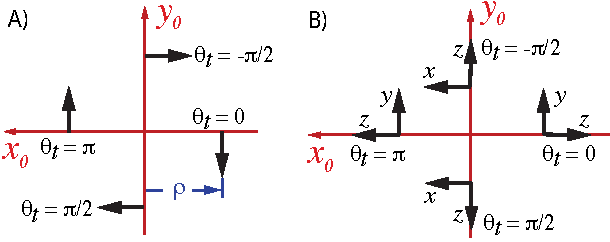
\includegraphics{tilt-bend.pdf} 
\caption[Orientation of a Bend.] 
  {
A) Rotation axes (bold arrows) for four different \vn{ref_tilt} angles of $\theta_t$ = 0, $\pm
\pi/2$, and $\pi$. $(x_0, y_0, z_0)$ are the machine coordinates at the entrance end of the bend with
the $z_0$ axis being directed into the page. Any rotation axis will be displaced by a distance of
the bend radius \vn{rho} from the origin. B) The $(x, y, z)$ coordinates at the exit end of the bend
for the same four \vn{ref_tilt} angles. In this case the bend angle is taken to be $\pi/2$.
  }
  \label{f:tilt.bend}
\end{figure}

%-----------------------------------------------------------------------

\index{rbend}\index{sbend}
\index{rho}\index{tilt}\index{angle}
For a \vn{bend}, the axis of rotation is dependent upon the bend's \vn{ref_tilt} angle
(\sref{s:offset}) as shown in \fig{f:tilt.bend}A. The axis of rotation points in the negative $y_0$
direction for \vn{ref_tilt} = 0 and is offset by the bend radius \vn{rho}. Here $(x_0, y_0, z_0)$
are the machine coordinates at the entrance end of the bend with the $z_0$ axis being directed into
the page in the figure.  For a non-zero \vn{ref_tilt}, the rotation axis is itself rotated about the
$z_0$ axis by the value of \vn{ref_tilt}. \fig{f:tilt.bend}B shows the exit coordinates for four
different values of \vn{ref_tilt} and for a bend angle \vn{angle} of $\pi/2$.  Notice that for a
bend in the horizontal $X-Z$ plane, a positive bend \vn{angle} will result in a decreasing azimuth
angle $\theta$.

For a bend, $\bfS$ is given using \Eq{wctux2} with 
\begin{align}
  \Bf u &= (-\sin\theta_t, -\cos\theta_t, 0) \CRNO
  \beta &= \alpha_b
  \label{ustt}
\end{align}
where $\theta_t$ is the \vn{ref_tilt} angle. The $\bfL$ vector for a \vn{bend} is given by 
\begin{equation}
  \bfL = \bfR_{z}(\theta_t) \; \bftilde L, \quad
  \bftilde L = 
  \begin{pmatrix}
    \rho (\cos\alpha_b - 1) \\ 0 \\ \rho \, \sin\alpha_b
  \end{pmatrix}
  \label{lrztt}
\end{equation}
where $\alpha_b$ is the bend \vn{angle} (\sref{s:bend}) and $\rho$ being the bend radius
(\vn{rho}). Notice that since $\Bf u$ is perpendicular to $z$, the curvilinear reference coordinate
system has no ``torsion''. That is, it is a Frenet-Serret coordinate system.

Note: An alternative equation for \vn{\bfS} for a bend is
 \begin{equation}
  \bfS = \bfR_{z}(\theta_t) \; \bfR_{y}(-\alpha_b) \; \bfR_{z}(-\theta_t)
  \label{srrr}
\end{equation}

The bend transformation above is so constructed that the transformation is equivalent to rotating
the machine coordinate system around an axis that is perpendicular to the plane of the bend. This
rotation axis is invariant under the bend transformation. For example, for $\theta_t = 0$ (or $\pi$)
the $y$-axis is the rotation axis and the $y$-axis of the machine coordinates before the bend will be
parallel to the $y$-axis of the machine coordinates after the bend as shown in \fig{f:tilt.bend}. That
is, a lattice with only bends with $\theta_t = 0$ or $\pi$ will lie in the horizontal plane (this
assuming that the $y$-axis starts out pointing along the $Y$-axis as it does by default).  For
$\theta_t = \pm\pi/2$, the bend axis is the $x$-axis. A value of $\theta_t = +\pi/2$ represents a
downward pointing bend.

\begin{figure}
  \centering 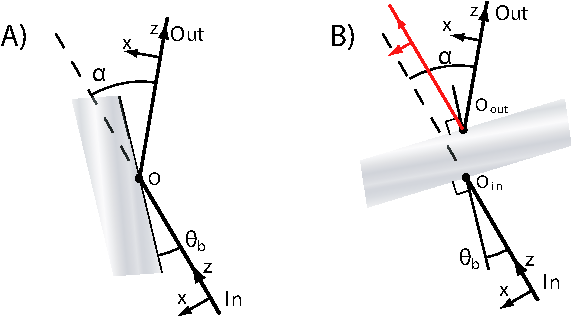
\includegraphics{mirror.pdf} 
\caption[Mirror and crystal geometry] {Mirror and crystal geometry.  The geometry shown here is
appropriate for a \vn{ref_tilt} angle of $\theta_t = 0$.  $\theta_g$ is the bend angle of the
incoming (entrance) ray, and $\alpha_b$ is the total bend angle of the reference trajectory. A)
Geometry for a mirror or a Bragg crystal. Point $\calO$ is the origin of both the machine coordinates
just before and just after the reflection/diffraction. B) Geometry for a Laue crystal.  Point
$\calO_{out}$ is the origin of the coordinates just after diffraction is displaced from the origin
$\calO_{in}$ just before diffraction due to the finite thickness of the crystal. here the bend
angles are measured with respect to the line that is in the plane of the entrance and exit
coordinates and perpendicular to the surface. For Laue diffraction, the user has the option of using
the undiffracted beam (shown in red) as the reference trajectory.
  }  
  \label{f:mirror}
\end{figure}

%-----------------------------------------------------------------------------
\subsection{Position Transformation When Transforming Coordinates}
\label{s:pos.trans}

A point $\bfQ_g = (X, Y, Z)$ defined in the global coordinate system, when expressed in the
coordinate system defined by $(\bfV, \bfW)$ is
\begin{equation}
  \bfQ_{VW} = \bfW^{-1} \left( \bfQ_g - \bfV \right)
  \label{rwrv}
\end{equation}
This is essentially the inverse of \Eq{vwlv}. That is, vectors propagate inversely to the
propagation of the coordinate system.

Using \Eq{rwrv} with \Eqs{vwlv}, and \eq{wws}, the transformation of a particle's position $\bfq =
(x,y,z)$ and momentum $\bfP = (P_x, P_y, P_z)$ when the coordinate frame is transformed from frame
$(\bfV_{i-1}, \bfW_{i-1})$ to frame $(\bfV_i, \bfW_i)$ is
\begin{align}
  \bfq_i &= \bfS_i^{-1} \, \left( \bfq_{i-1} - \bfL_i \right), 
    \label{rwlr} \\
  \bfP_i &= \bfS_i^{-1} \, \bfP_{i-1}
    \label{pps}
\end{align}

Notice that since $\bfS$ (and $\bfW$) is the product of orthogonal rotation matrices, $\bfS$ is
itself orthogonal and its inverse is just the transpose
\begin{equation}
  \bfS^{-1} = \bfS^T
\end{equation}

%-----------------------------------------------------------------------------
\subsection{Crystal and Mirror Element Coordinate Transformation}
\label{s:mirror.coords}

\index{crystal}\index{mirror}\index{ref_tilt}
A \vn{crystal} element (\sref{s:mirror}) diffracts photons and a \vn{mirror} element
(\sref{s:mirror}) reflects them. For a crystal setup for Bragg diffraction, and for a mirror, the
reference orbit is modeled as a zero length bend with $\bftilde L = (0, 0, 0)$, as shown in
\fig{f:mirror}A. Shown in the figure is the geometry appropriate for a \vn{ref_tilt} angle of
$\theta_t = 0$ (the rotation axis is here the $y$-axis). Since the mirror or crystal element is
modeled to be of zero length, the origin points (marked $\calO$ in the figure) of the entrance and
exit machine coordinates are the same. For Laue diffraction, the only difference is that $\bftilde L$
is non-zero due to the finite thickness of the crystal as shown in \fig{f:mirror}B. This results in
a separation between the entrance coordinate origin $\calO_{in}$ and the exit coordinate origin
$\calO_{out}$.

In all cases, the total bending angle is
\begin{align}
  \alpha_b &= \text{bragg_angle_in} + \text{bragg_angle_out} &&
                  \text{! Crystal, graze_angle_in} = 0 \CRNO
  \alpha_b &= \text{graze_angle_in} + \text{graze_angle_out} &&
                   \text{! Crystal, graze_angle_in} \ne 0 \CRNO
  \alpha_b &= 2 \, \text{graze_angle}                        &&\text{! Mirror}
  \label{agg}
\end{align}
With a mirror or Bragg diffraction, the bend angles are measured with respect to the surface
plane. With Laue diffraction the bend angles are measured with respect to the line in the bend plane
perpendicular to the surface.

For Laue diffraction, the user has the option of using the undiffracted beam (shown in red) as the
reference trajectory.

The orientation of the exit coordinates (the machine coordinates after the reflection) are only
affected by the element's \vn{ref_tilt} and bend angle parameters and is independent of all other
parameters such as the radius of curvature of the surface, etc. The machine $z$-axis of the entrance
coordinates along with the $z$-axis of the exit coordinates define a plane which is called the
element's \vn{bend plane}.  For a mirror, the graze angle is a parameter supplied by the user. For a
crystal, the Bragg angles are calculated so that the reference trajectory is in the middle of the
Darwin curve. Calculation of the Bragg angles for a crystal is given in
Section~\sref{s:crystal.ref}.

%-----------------------------------------------------------------------------
\subsection{Patch and Floor_Shift Elements Entrance to Exit Transformation}
\label{s:patch.coords}

\index{patch!coordinate transformation}\index{floor_shift!coordinate transformation}
For \vn{patch} (\sref{s:patch}) and \vn{floor_shift} (\sref{s:floor.ele}) elements, the shift in the
exit end reference coordinates is given by \Eqs{vwlv} and \eq{wws} with
\begin{align}
  \bfL &= 
    \begin{pmatrix} 
      \text{x_offset} \\ \text{y_offset} \\ \text{z_offset} 
    \end{pmatrix}
    \CRNO
  \bfS &= \bfR_{y} (\text{y_rot}) \; \bfR_{x} (\text{y_rot}) \; \bfR_{z} (\text{tilt})
  \label{swww}
\end{align}

The difference here between \vn{patch} and \vn{floor_shift} elements is that, with a \vn{patch}
element, the shift is relative to the exit end of the previous element while, for a \vn{floor_shift}
element, the shift is relative to the reference point on the origin element specified by the
\vn{origin_ele} parameter of the \vn{floor_shift}.

%-----------------------------------------------------------------------------
\subsection{Fiducial and Girder Elements Origin Shift Transformation}
\label{s:girder.coords}

\index{girder}\index{fiducial}
For \vn{fiducial} and \vn{girder} elements, the alignment of the
reference coordinates with respect to ``\vn{origin}'' coordinates is
analogous to \Eqs{swww}. Explicitly:
\begin{align}
  \bfL &= 
    \begin{pmatrix} 
      \text{dx_origin} \\ \text{dy_origin} \\ \text{dz_origin}
    \end{pmatrix}
    \CRNO
  \bfS &= \bfR_{y} (\text{dtheta_origin}) \; \bfR_{-x} (\text{dphi_origin}) \; 
    \bfR_{z} (\text{dpsi_origin})
\end{align}

%-----------------------------------------------------------------------------
\subsection{Reflection Patch}
\label{s:reflect.patch}
\index{patch!reflection}

A \vn{Patch} (or a series of patches) that reflects the direction of the \vn{z}-axis is called a
\vn{reflection} \vn{patch}. By ``reflected direction'' it is meant that the dot product $\Bf z_1
\cdot \Bf z_2$ is negative where $\Bf z_1$ is the $z$-axis vector at the \vn{entrance} face and $\Bf
z_2$ is the $z$-axis vector at the \vn{exit} face. This condition is equivalent to the condition
that the associated $\bfS$ matrix (see \Eq{swww}) satisfy:
\begin{equation}
  S(3,3) < 0
  \label{s330}
\end{equation}
Using \Eq{swww} gives, after some simple algebra, this condition is equivalent to
\begin{equation}
  \cos(\text{x_rot}) \, \cos(\text{y_rot}) < 0
\end{equation}
When there are a series of patches, The transformations of all the patches are concatenated together
to form an effective $\bfS$ which can then be used with \Eq{s330}.

%-----------------------------------------------------------------------------
\section{Transformation Between Machine and Element Body Coordinates}
\label{s:lab.body.transform}
\index{machine coordinates}
\index{element body coordinates|hyperbf}

The \vn{element body} coordinates are the coordinate system attached to an element. Without any
misalignments, where \vn{``misalignments''} are here defined to be any offset, or rotation
(\sref{s:offset}), the \vn{machine} coordinates (\sref{s:ref}) and \vn{element body} coordinates
are the same. With misalignments, the transformation between \vn{machine} and \vn{element body}
coordinates depends upon whether the machine coordinate system is straight (\sref{s:straight.mis}) or
bent (\sref{s:bend.mis}).

When tracking a particle through an element, the particle starts at the \vn{nominal}
(\sref{s:coords}) upstream end of the element with the particle's position expressed in machine
coordinates. Tracking from the the nominal upstream end to the actual upstream face of the element
involves first transforming to element body coordinates (with $s = 0$ in the equations below) and
then propagating the particle as in a field free drift space from the particle's starting position
to the actual element face. Depending upon the element's orientation, this tracking may involve
tracking backwards. Similarly, after a particle has been tracked through the physical element to the
actual downstream face, the tracking to the nominal downstream end involves transforming to
machine coordinates (using $s = L$ in the equations below) and then propagating the particle as
in a field free drift space to the nominal downstream edge.

%-----------------------------------------------------------------------------
\subsection{Straight Element Misalignment Transformation}
\label{s:straight.mis}

For straight line elements, given a machine coordinate frame $\Lambda_s$ with origin a distance
$s$ from the beginning of the element, misalignments will shift the coordinates to a new reference
frame denoted $E_s$. Since misalignments are defined with respect to the middle of the element, the
transformation between $\Lambda_s$ and $E_s$ is a three step process:
\begin{equation}
  \Lambda_s \longrightarrow \Lambda_\text{mid} 
  \longrightarrow E_\text{mid} \longrightarrow E_s
  \label{llee}
\end{equation}
where $\Lambda_\text{mid}$ and $E_\text{mid}$ are the machine and element reference frames at the
center of the element.

The first and last transformations from $\Lambda_s$ to $\Lambda_\text{mid}$ and from $E_\text{mid}$
to $E_s$ use \Eqs{vwlv}, \eq{wws}, and \eq{l00l} with the replacement $L \rightarrow L/2 - s$ for
the first transformation and $L \rightarrow s - L/2$ for the third transformation. The middle
transformation, by definition of the offset and rotation parameters is
\begin{align}
  \bfL &= 
    \begin{pmatrix} 
      \text{x_offset} \\ \text{y_offset} \\ \text{z_offset} 
    \end{pmatrix}
    \CRNO
  \bfS &= \bfR_{y} (\text{x_rot}) \; \bfR_{x} (\text{y_rot}) \; \bfR_{z} (\text{tilt})
  \label{swww2}
\end{align}

Notice that with this definition of how elements are misaligned, the position of the center of a
non-bend misaligned element depends only on the offsets, and is independent of the rotations.

%-----------------------------------------------------------------------------
\subsection{Bend Element Misalignment Transformation}
\label{s:bend.mis}

This needs cleanup!!!

\index{rbend!coordinate transformation}\index{sbend!coordinate transformation}
\index{roll!coordinate transformation}\index{tilt!coordinate transformation}
For \vn{rbend} and \vn{sbend} elements there is no \vn{tilt} parameter.  Rather, there is the
\vn{roll} parameter and a \vn{ref_tilt} parameter. The latter affects both the reference orbit and
the bend position (\sref{s:bend.orient}). Furthermore, \vn{ref_tilt} is calculated with respect to
the coordinates at the beginning of the bend while, like straight elements, \vn{roll}, \vn{x_rot},
\vn{y_rot}, and offsets are calculated with respect to the center of the bend. 
The different reference frame used
for \vn{ref_tilt} versus everything else means that five transformations are needed to get from the
machine frame to the element body frame (see \Eq{llee}). Symbolically:
\begin{equation}
  \Lambda_s \longrightarrow \Lambda_\text{mid} 
  \longrightarrow \Omega_\text{mid} \longrightarrow \Omega_0
  \longrightarrow E_0 \longrightarrow E_s
\end{equation}

The first transformation, $\Lambda_s$ to $\Lambda_\text{mid}$, from machine coordinates at a
distance $s$ from the beginning of the element to machine coordinates at the center the bend is a
rotation around the center of curvature of the bend and is given by \Eqs{vwlv} and \eq{wws} with
\Eqs{ustt} and \eq{lrztt} with the substitution $\alpha_b \rightarrow (L/2 - s)/\rho$.

The second transformation $\Lambda_\text{mid}$ to $\Omega_\text{mid}$ at the center of the element
adds in the misalignments (Note that the coordinate frame $\Omega_\text{mid}$ is neither a
machine frame or an element frame so hence the use of a different symbol $\Omega$). Explicitly,
the $\Lambda_\text{mid} \longrightarrow \Omega_\text{mid}$ transformation is
\begin{align}
  \bfL &= \bfL_\text{off} + 
    \left[ \bfR_z(\text{roll}) - \Bf1 \right] \; \bfR_z(\theta_t) \; \bfR_{y}(\alpha_b/2) \; 
      \bfL_c \CRNO
  \bfS &= \bfR_{y}(\text{y_rot}) \; \bfR_{x}(\text{x_rot}) \; \bfR_z(\text{roll})
  \label{lcmis}
\end{align}
where
\begin{equation}
  \bfL_c = 
    \begin{pmatrix}
      \rho (\cos(\alpha_b/2) - 1) \\ 0 \\ \rho \, \sin(\alpha_b/2)
    \end{pmatrix}
  , \qquad
  \bfL_\text{off} = 
    \begin{pmatrix} 
      \text{x_offset} \\ \text{y_offset} \\ \text{z_offset} 
    \end{pmatrix}
\end{equation}
The reason why $\bfL$ has a different form from straight line elements is due to the fact that the
axis of rotation for a \vn{roll} is displaced from the $z$-axis of the coordinate system at the
center of the bend (see \fig{f:roll}).

The third transformation from $\Omega_\text{mid}$ to $\Omega_0$ is like the first transformation and
rotates from the center of the bend to the beginning. Again \Eqs{ustt} and \eq{lrztt} are used with
the substitution $\alpha_b \rightarrow -L/2\rho$.

The fourth transformation $\Omega_0$ to $E_0$ tilts the reference frame by an amount \vn{ref_tilt}:
\begin{equation}
  \bfL = 0, \quad
  \bfS = \bfR_{z}(\theta_t)
  \label{l0sr}
\end{equation}

The fifth and final transformation, $E_0$ to $E_s$, like the first and third, rotates around the
center of the bend but in this case, since we are dealing with element coordinates, the
\vn{ref_tilt} is ignored.  That is, \Eqs{ustt} and \eq{lrztt} are used with the substitutions
$\theta_t \rightarrow 0$ and $\alpha_b \rightarrow L/\rho$.

Notice that with this definition of how elements are misaligned, the position of the center of a
misaligned element depends only on the offsets and \vn{roll}, and is independent of any rotations. 
Also the orientation of an element depends only on the \vn{x_rot}, \vn{y_rot}, \vn{roll}, 
and \vn{ref_tilt}, and is independent of the offsets.

%-----------------------------------------------------------------------------
\section{Phase Space Coordinates}
\label{s:phase.coords}
\index{phase space coordinates|hyperbf}

%-----------------------------------------------------------------------------
\subsection{Reference Particle, Reference Energy, and Reference Time}
\label{s:ref.energy}
\index{reference particle|hyperbf}
\index{reference energy|hyperbf}
\index{reference time|hyperbf}

The \vn{reference energy} and \vn{reference time} are needed in evaluating the phase space
coordinates of charged particles (\sref{s:phase.space}).

All lattice elements, except for controller elements, have an associated \vn{reference energy}
energy.  The reference energy at the start of a lattice's \vn{root branch} (\sref{s:branch.def}) is
set in the lattice file by setting the reference momentum (\vn{p0c}) or total energy (\vn{E_tot})
using a \vn{parameter} (\sref{s:param}) or \vn{beginning} (\sref{s:beginning}) statement. For other
branches, the energy at the start of the branch is set using the appropriate line parameter
(\sref{s:beginning}) statement.

Note that the reference momentum \vn{p0c} is actually the reference momentum times the speed of light
so that the reference momentum has the same unit (eV) as the reference energy.

\index{custom!reference energy}\index{em_field!reference energy}
\index{hybrid!reference energy}\index{lcavity!reference energy}
\index{patch!reference energy}
For most elements, the reference energy is the same as the reference energy of the proceeding
element. The following elements are exceptions:
\begin{example}
  custom
  em_field
  hybrid
  lcavity
  patch
\end{example}
The reference energy of these elements is determined by tracking a particle (the ``\vn{reference
particle}'') through the element with the particle starting on the reference orbit and whose energy
is equal to the reference energy. The energy of the particle at the downstream end is the reference
energy of the element. Note: Tracking through an element to determine the reference energy is always
done with the element turned on independent of the setting of the element's \vn{is_on}
(\sref{s:is.on}) parameter. Reference energy tracking is also done ignoring any orientation parameters
(\sref{s:offset}) and errors like \vn{voltage_err}.

\index{wiggler!reference time}
Besides the reference energy, lattice elements have an associated \vn{reference time} which is
computed, for most elements, by the time-of-flight of the \vn{reference particle} assuming that the
reference particle is following the reference orbit. Exceptions are \vn{wiggler} elements which uses
the time-of-flight of the actual undulating trajectory. [Actually what is used in the computation of
the $z$ phase space coordinate (\Eq{zbctt}) is the sum of reference time deltas of the elements that
a particle has passed through. It is not possible to assign a unique reference time to an element
when particles are recirculating through elements as in a storage ring.]

%-----------------------------------------------------------------------------
\subsection{Charged Particle Phase Space Coordinates}
\label{s:phase.space}
\index{phase space coordinates|hyperbf}

\begin{figure}
\centering 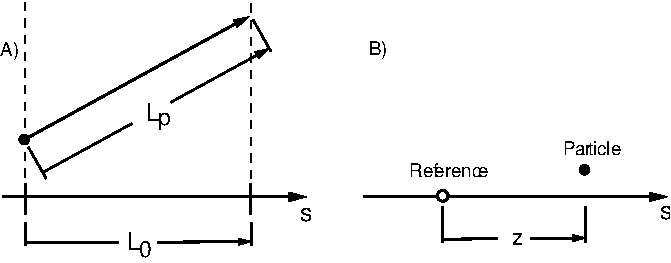
\includegraphics{canonical-z.pdf} \caption[Interpreting phase space $z$ at constant
velocity.]  {Interpreting phase space $z$ at constant velocity: A) The change in $z$ going through
an element of length $L_0$ is $L_0 - L_p$.  B) At constant time, $z$ is the longitudinal distance
between the reference particle and the particle.}  \label{f:canonical.z}
\end{figure}

For charged particles (more correctly, for everything but photons (\sref{s:photon.phase.space})),
\bmad uses the canonical phase space coordinates
\begin{equation}
  \Bf r(s) = (x, p_x, y, p_y, z, p_z)
\end{equation}
The longitudinal position $s$ is the independent variable instead of the time. $x$ and $y$, are the
transverse coordinates of the particle as shown in~\fig{f:machine.coords}A. Note that $x$ and $y$ are
independent of the position of the reference particle.

The phase space momenta $p_x$ and $p_y$ are normalized by the reference (sometimes called the
design) momentum $P_0$
\begin{equation}
  p_x = \frac{P_x}{P_0}, \qquad
  p_y = \frac{P_y}{P_0}
  \label{ppp}
\end{equation}
where $P_x$ and $P_y$ are respectively the $x$ and $y$ momentums.

\index{lcavity}\index{rfcavity}
The phase space $z$ coordinate is 
\begin{align}
  z(s) &= -\beta(s) \, c \, (t(s) - t_0(s)) \CRNO
    &\equiv - \beta(s) \, c \, \Delta t(s)
  \label{zbctt}
\end{align}
$t(s)$ is the time at which the particle is at position $s$, $t_0(s)$ is the time at which the
reference particle is at position $s$, and $\beta$ is $v/c$ with $v$ being the particle velocity
(and not the reference velocity). The reference particle is, by definition, ``synchronized'' with
elements whose fields are oscillating and therefore the actual fields a particle will see when
traveling through such an element will depend upon the particle's phase space $z$. For example, the
energy change of a particle traveling through an \vn{lcavity} (\sref{s:lcav}) or \vn{rfcavity}
(\sref{s:rfcav}) element is $z$ dependent. Exception: With absolute time tracking (\sref{s:rf.time})
fields are tied to the absolute time and not $z$.

If the particle's velocity is constant, and is the same as the velocity of the reference particle
(for example, at high energy where $\beta = 1$ for all particles), then $\beta \, c \, t$ is just
the path length. In this case, the change in $z$ going through an element is
\begin{equation}
  \Delta z = L_0 - L_p
\end{equation}
where, as shown in \fig{f:canonical.z}A, $L_0$ is the path length of the reference particle (which
is just the length of the element) and $L_p$ is the path length of the particle in traversing the
element.  Another way of interpreting phase space $z$ is that, at constant $\beta$, and constant
time, $z$ is the longitudinal distance between the particle and the reference particle as shown in
\fig{f:canonical.z}B. with positive $z$ indicating that the particle is ahead of the reference
particle.

Do not confuse the phase space $z$ with the $z$ that is the particle's longitudinal coordinate in
the machine reference frame as shown in \fig{f:machine.coords}. By construction, this latter $z$ is
always zero.

Notice that if a particle gets an instantaneous longitudinal kick so that $\beta$ is discontinuous
then, from \Eq{zbctt}, phase space $z$ is discontinuous even though the particle itself does not
move in space. In general, from \Eq{zbctt}, The value of $z$ for a particle at $s_2$ is related to
the value of $z$ for the particle at $s_1$ by
\begin{equation}
  z_2 = \frac{\beta_2}{\beta_1} \, z_1 - 
  \beta_2 \, c \, (\Delta t_2 - \Delta t_1)
  \label{zbbzb}
\end{equation}
$\Delta t_2 - \Delta t_1$ can be interpreted as the difference in transit time, between the particle
and the reference particle, in going from $s_1$ to $s_2$.

The longitudinal phase space momentum $p_z$ is given by
\begin{equation}
  p_z = \frac{\Delta P}{P_0} \equiv \frac{P - P_0}{P_0}
  \label{ppppp}
\end{equation}
where $P$ is the momentum of the particle. For ultra--relativistic particles $p_z$ can be
approximated by
\begin{equation}
  p_z = \frac{\Delta E}{E_0}
\end{equation}
\index{lcavity}
where $E_0$ is the reference energy (energy here always refers to the total energy) and $\Delta E =
E - E_0$ is the deviation of the particle's energy from the reference energy. For an \vn{Lcavity}
element (\sref{s:lcav}) the reference momentum is {\it not} constant so the tracking for an
\vn{Lcavity} is not canonical.

\index{phase space coordinates!MAD convention}
\index{MAD!phase space convention}
\mad uses a different coordinate system where $(z, p_z)$ is replaced by $(-c\Delta t, p_t)$ where
$p_t \equiv \Delta E / P_0 c$. For highly relativistic particles the two coordinate systems are
identical.

\index{paraxial approximation}
\index{bmad_standard!tracking method}
The relationship, between the phase space momenta and the slopes $x' \equiv dx/ds$ and 
$y' \equiv dy/ds$ is
\begin{align}
  x' &= \frac{p_x}{\sqrt{(1 + p_z)^2 - p_x^2 - p_y^2}} \, (1 + g x) \\
  y' &= \frac{p_y}{\sqrt{(1 + p_z)^2 - p_x^2 - p_y^2}} \, (1 + g x) 
  \label{xpa1p}
\end{align}
$g = 1/\rho$ is the curvature function with $\rho$ being the radius of curvature of the reference
orbit and it has been assumed that the bending is in the $x$--$z$ plane.

With the paraxial approximation, and in the relativistic limit, the change in $z$ with position is
\begin{equation}
  \frac{dz}{ds} = -g \, x - \frac{1}{2} (x'^2 + y'^2)
\end{equation}
This shows that in a linac, without any bends, the $z$ of a particle always decreases.

A particle can also have a spin. The spin is characterized by the spinor $\Psi = \left( \psi_{1},
\psi_{2} \right)^{T}$ where $\psi_{1,2}$ are complex numbers (\sref{s:spin.dyn}).

%-----------------------------------------------------------------------------
\subsection{Time-based Phase Space Coordinates}
\label{s:time.phase.space}
\index{time!phase space coordinates|hyperbf}

Some specialized routines (for example, time Runge Kutta tracking) use the time $t$ as the
independent variable for charged particle tracking. This is useful when particles can reverse
direction since the normal $z$ based tracking cannot handle this. Direction reversal can happen, for
example, with low energy ``dark current'' electrons that are generated at the walls of the vacuum
chamber.

When the tracking is time based the phase space coordinates are:
\begin{equation}
  (x, c \, p_x, y, c \, p_y, z, c \, p_s)
\end{equation}
The positions $x$, $y$, and $z$ are the same as with phase space coordinates
(\sref{s:phase.space}). The momenta are defined as
\begin{align}
c p_x &\equiv m c^2 \gamma \beta_x \CRNO
c p_y &\equiv m c^2 \gamma \beta_y \\
c p_s &\equiv m c^2 \gamma \beta_s, \nonumber
\end{align}
and internally are stored in units of eV.

%-----------------------------------------------------------------------------
\subsection{Photon Phase Space Coordinates}
\label{s:photon.phase.space}
\index{photon!phase space coordinates|hyperbf}

The phase space coordinates discussed above implicitly assume that
particles are traveling longitudinally in only one direction. That is,
the sign of the $s$ component of the momentum cannot be determined
from the phase space coordinates. This is generally fine for tracking
high energy beams of charged particles but for photon tracking this
would oftentimes be problematical. For photons, therefore, a different
phase space is used:
\begin{equation}
  (x, \beta_x, y, \beta_y, z, \beta_z)
  \label{xbybzb}
\end{equation}
Here $(\beta_x, \beta_y, \beta_z)$ is the normalized photon velocity with
\begin{equation}
  \beta_x^2 + \beta_y^2 + \beta_z^2 = 1 
  \label{bbb1}
\end{equation}
and $(x, y, z)$ are the reference orbit coordinates with $z$ being the
distance from the start of the lattice element the photon is in.

In \bmad, the information associated with a photon include its phase
space coordinates and time along with the photon energy and four
parameters $E_x, \phi_x$, and $E_y, \phi_y$ specifying the intensity
and phase of the field along the $x$ and $y$ axes transverse to the
direction of propagation.  the field in the vicinity of the photon is
\begin{align}
  E_x (\Bf r, t) &\sim E_x \, e^{i (k \, (z - z_0) - \omega \, (t - t_\REF) + \phi_x)} \CRNO
  E_y (\Bf r, t) &\sim E_y \, e^{i (k \, (z - z_0) - \omega \, (t - t_\REF) + \phi_y)} 
  \label{ertee}
\end{align}
where $z_0$ is the photon $z$ position and and $t_\REF$ is the reference time.

The normalization between field and intensity is dependent upon the
particular parameters of any given simulation and so must be
determined by the program using \bmad.

